\subsection{Entrant al concepte del Cub de Rubik}

\subsubsection{Interpretar el concepte del cub}

Una gran majoria de la població ha tingut a les seves mans un cub de Rubik, i han intentat resoldre'l sense èxit. Això és totalment normal, ja que només el saben resoldre un 5,8\% de les persones que ho han intentat\cite{redbull-cub}.
\\\\Aquesta xifra es sol atribuir a la dificultat del cub, però després d'aprendre a fer el cub de rubik t'adones compte de què la raó no és aquesta. El fracàs a l'hora trobar la solució bé donat pel fet d'interpretar malament el concepte del funcionament del cub.
\\\\La majoria de les persones es pensa que el cub conté 54 "peces" de colors perquè calculen que per cada cara hi ha 9 peces i en un cub hi ha 6 cares, per tant estan treballant color a color.

$$ \textrm{Nº Quadrats} = 3\textrm{ Quadrats}*3\textrm{ Quadrats}*6\textrm{ Cares} = 54 $$

\begin{figure}[ht]
    \centering
    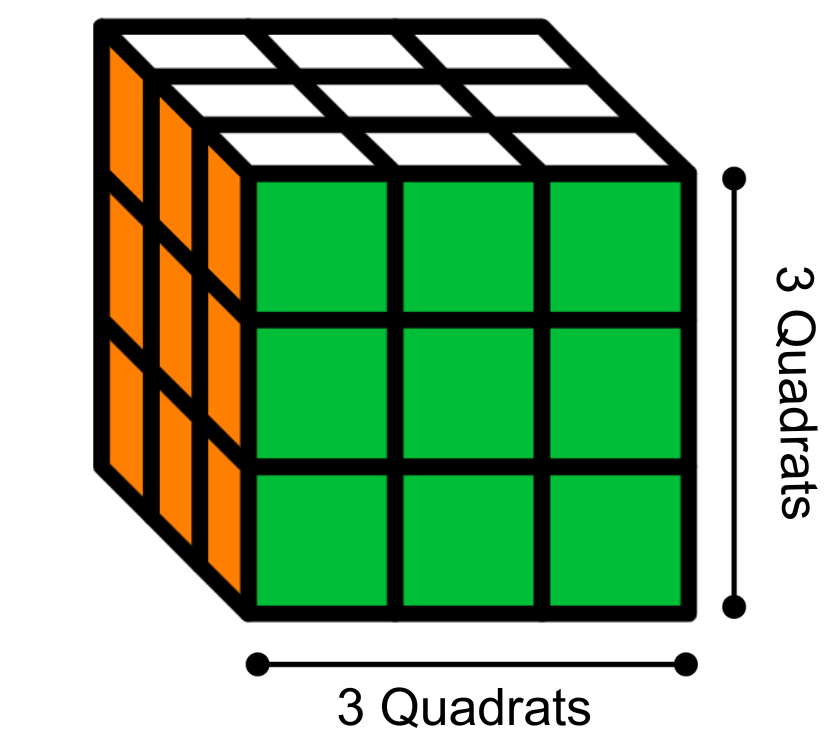
\includegraphics[width=7cm]{img/figures/plantejament-no.png}
    \caption{Plantejament típic però erroni del cub de rubik}
    \label{fig:plantejament-no}
\end{figure}

La manera correcta d'interpretar el cub és pensar en el funcionament, com si el desmuntessis, ja que consta de 12 arestes i 8 cantonades, a més a més dels 6 centres que no poden permutar\footnote{Intercanvi de posició amb una altre peça i de l'ordre de tot el conjunt} amb cap altra peça ja que només roten.

\begin{figure}[ht]
    \centering
    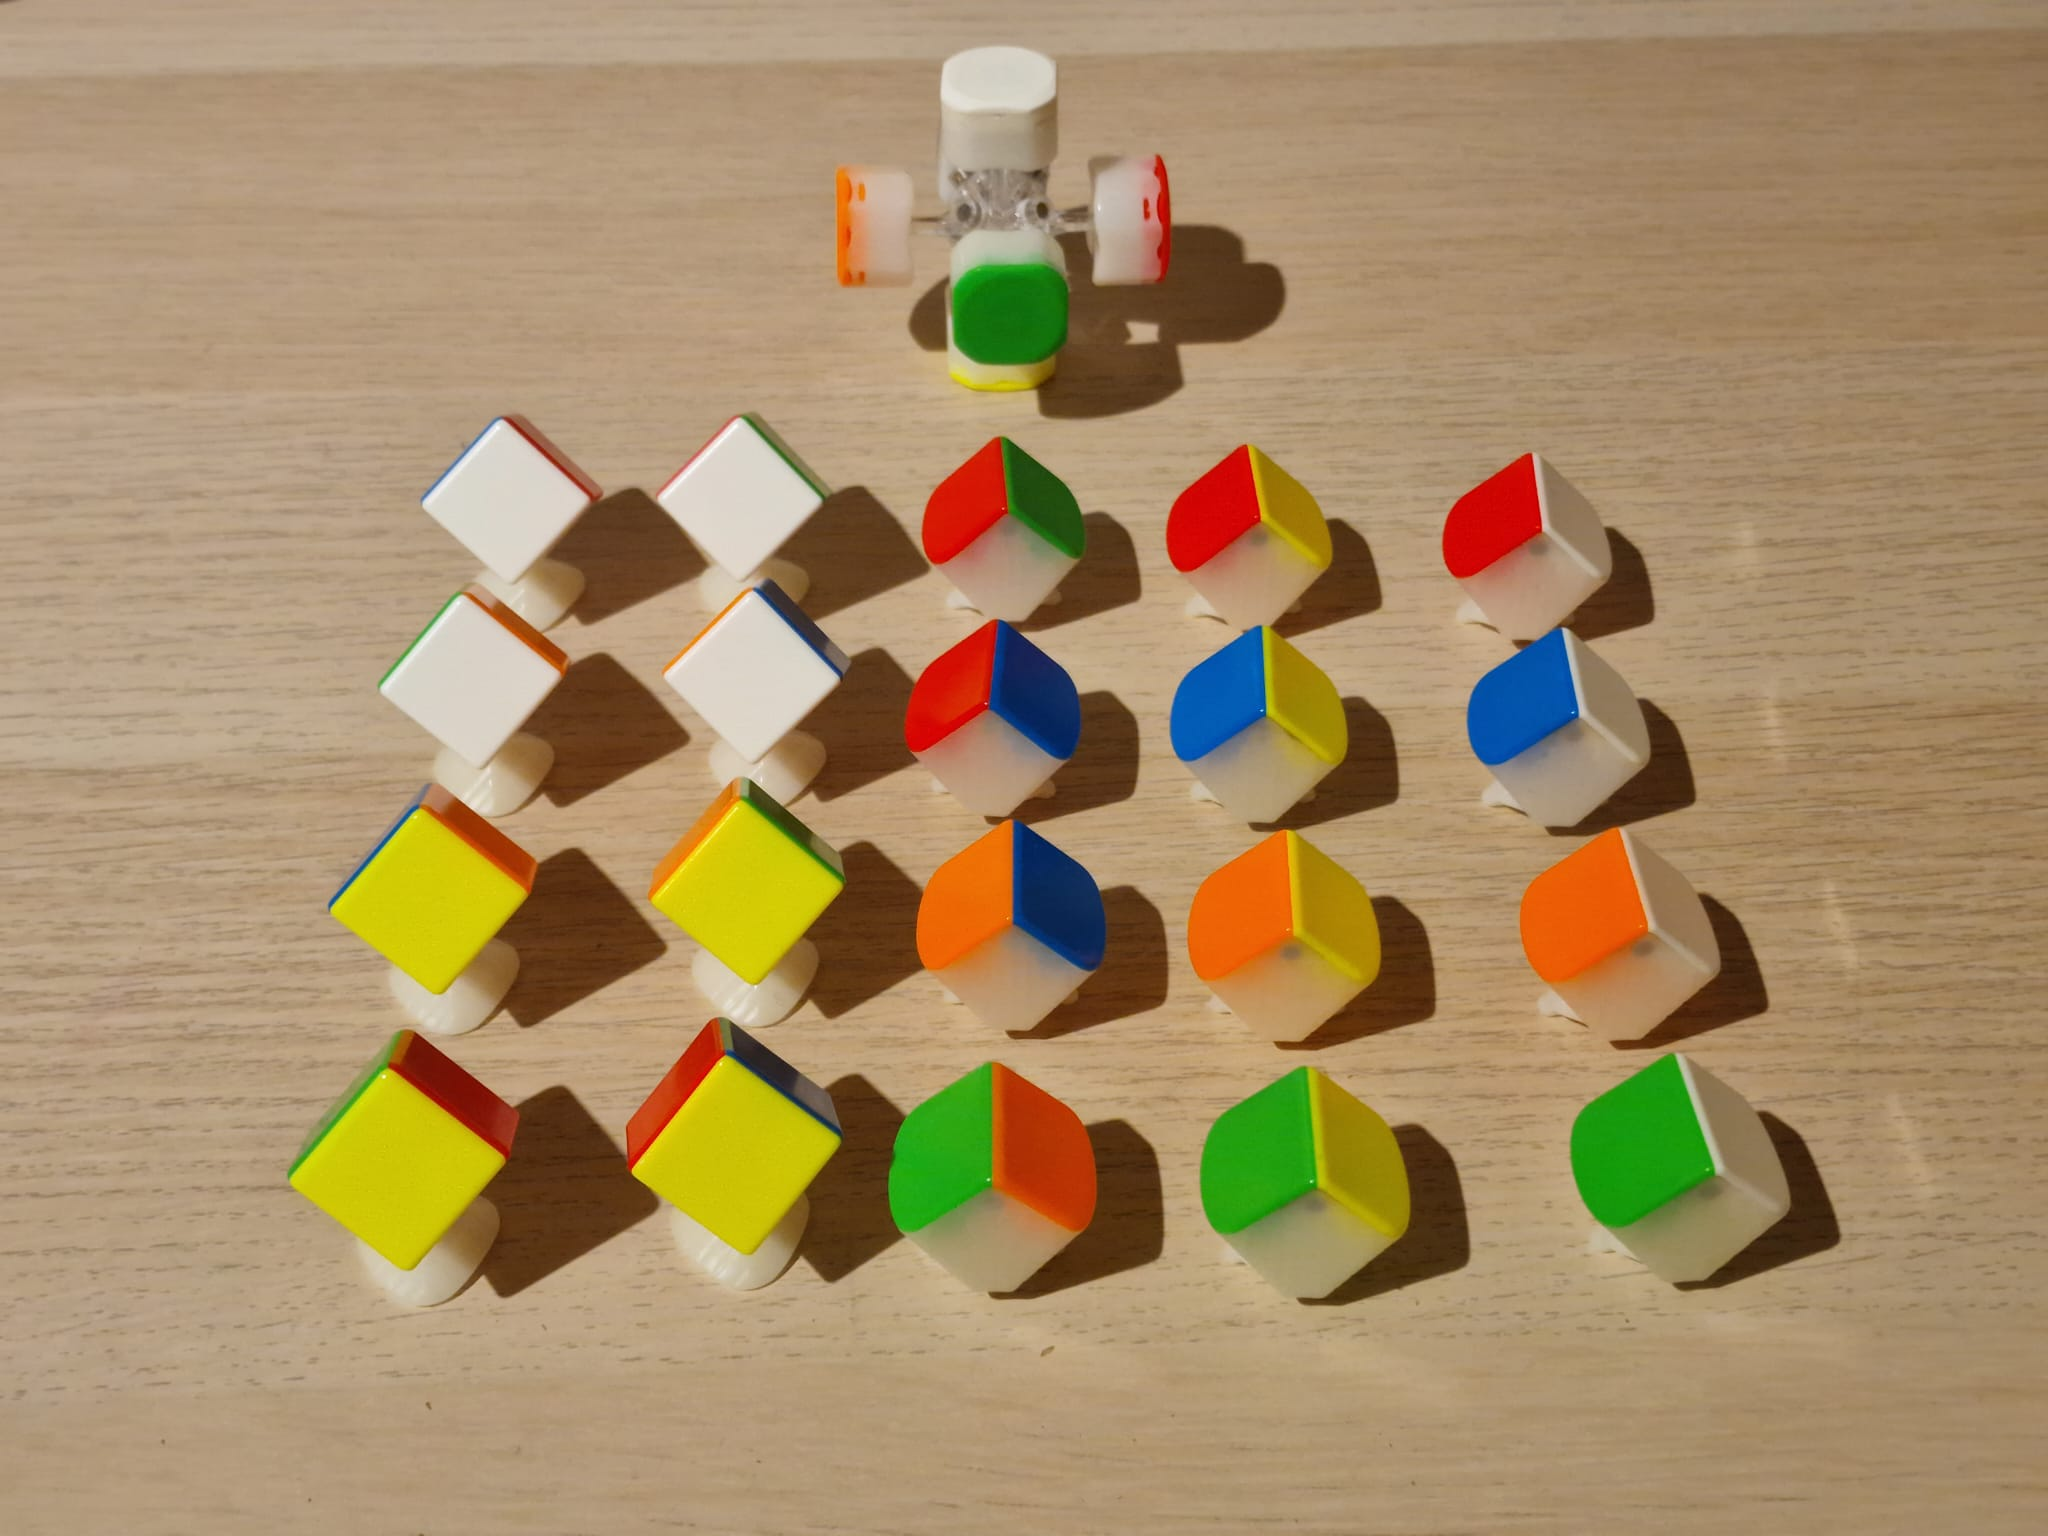
\includegraphics[width=7cm]{img/figures/cub-desmontat.jpg}
    \caption{Cub Desmuntat}
    \label{fig:cub-desmuntat}
\end{figure}

\subsubsection{Aplicar les matemàtiques al concepte}

Després d'entendre el funcionament podem aplicar les matemàtiques i extreure el nombre de combinacions possbiles del cub. En primer instant divid el càlcul el dos grups, per una part tenim cantonades i per l'altra arestes.
Per la part de les cantonades es calcula:
\\\\Tenim 8 cantonades que es poden posar de manera aleatoria en els 8 llocs, i això es calcula com a $ 8! $ \footnote{! és el símbol de factorial o $8*7*6*5*4*3*2*1$}, després aquestes es poden orientar en 3 direccions diferents que matemàticament és $ 3^8 $. Per tant les combinacions tèoriques possibles amb un cub de només cantonades són:

$$ \textrm{Nº Combinacions cantonades tèoric} = 8!*3^8 = 264.539.520 $$

\begin{figure}[h]
    \centering
    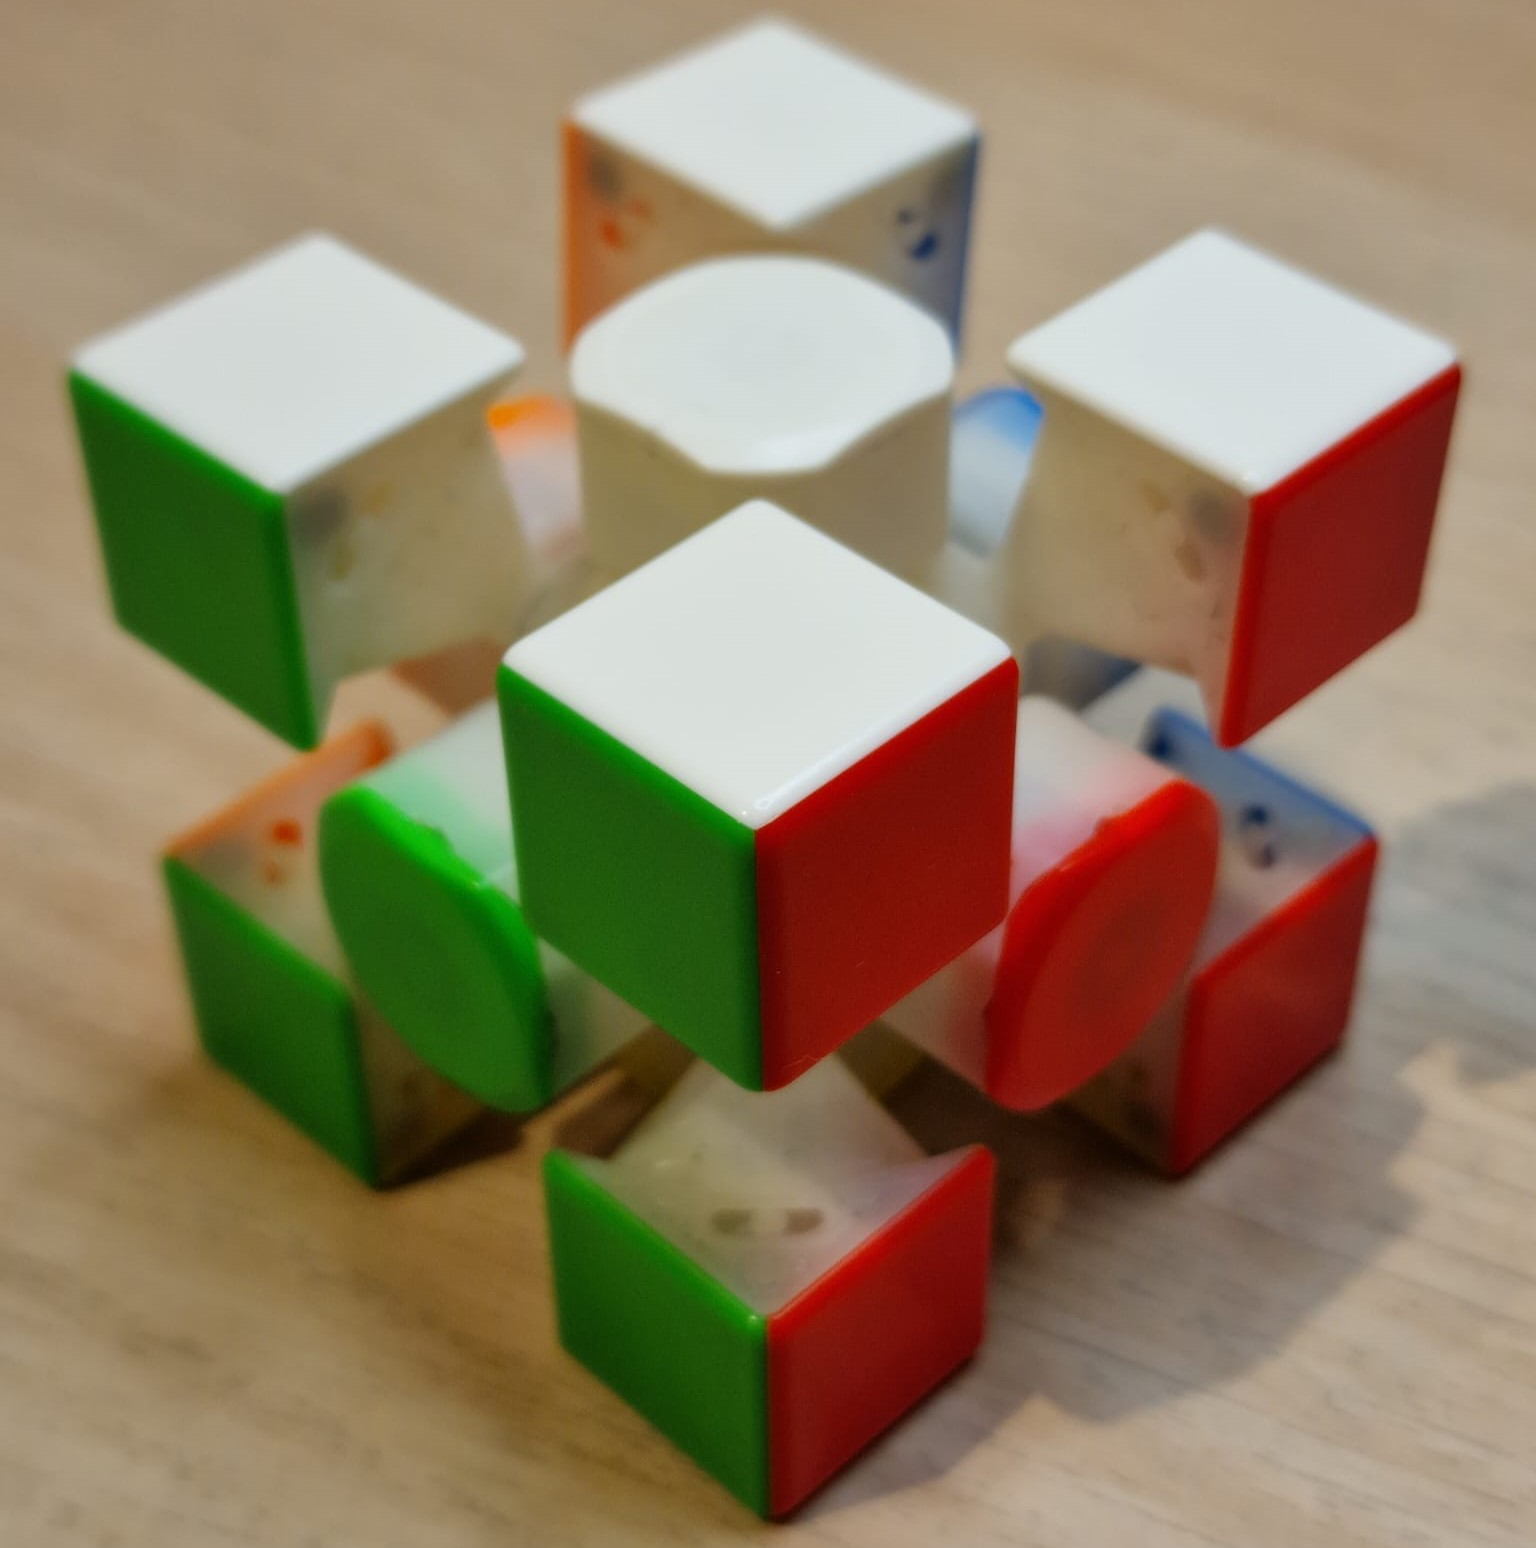
\includegraphics[width=5cm]{img/figures/only-corners.jpg}
    \caption{Cub amb només cantonades}
    \label{fig:only-corners}
\end{figure}
Per altra banda tenim 12 arestes que igual que amb les cantonades es calcula com a $ 12! $ i com que les arestes del cub només tenen dos orientacions ho multiplicarem per $2^12$. Per tant les combinacions tèoriques possibles amb un cub de només arestes són:  

$$ \textrm{Nº Combinacions arestes tèoric} = 12!*2^12 = 1.961.990.553.600$$

\begin{figure}[h]
    \centering
    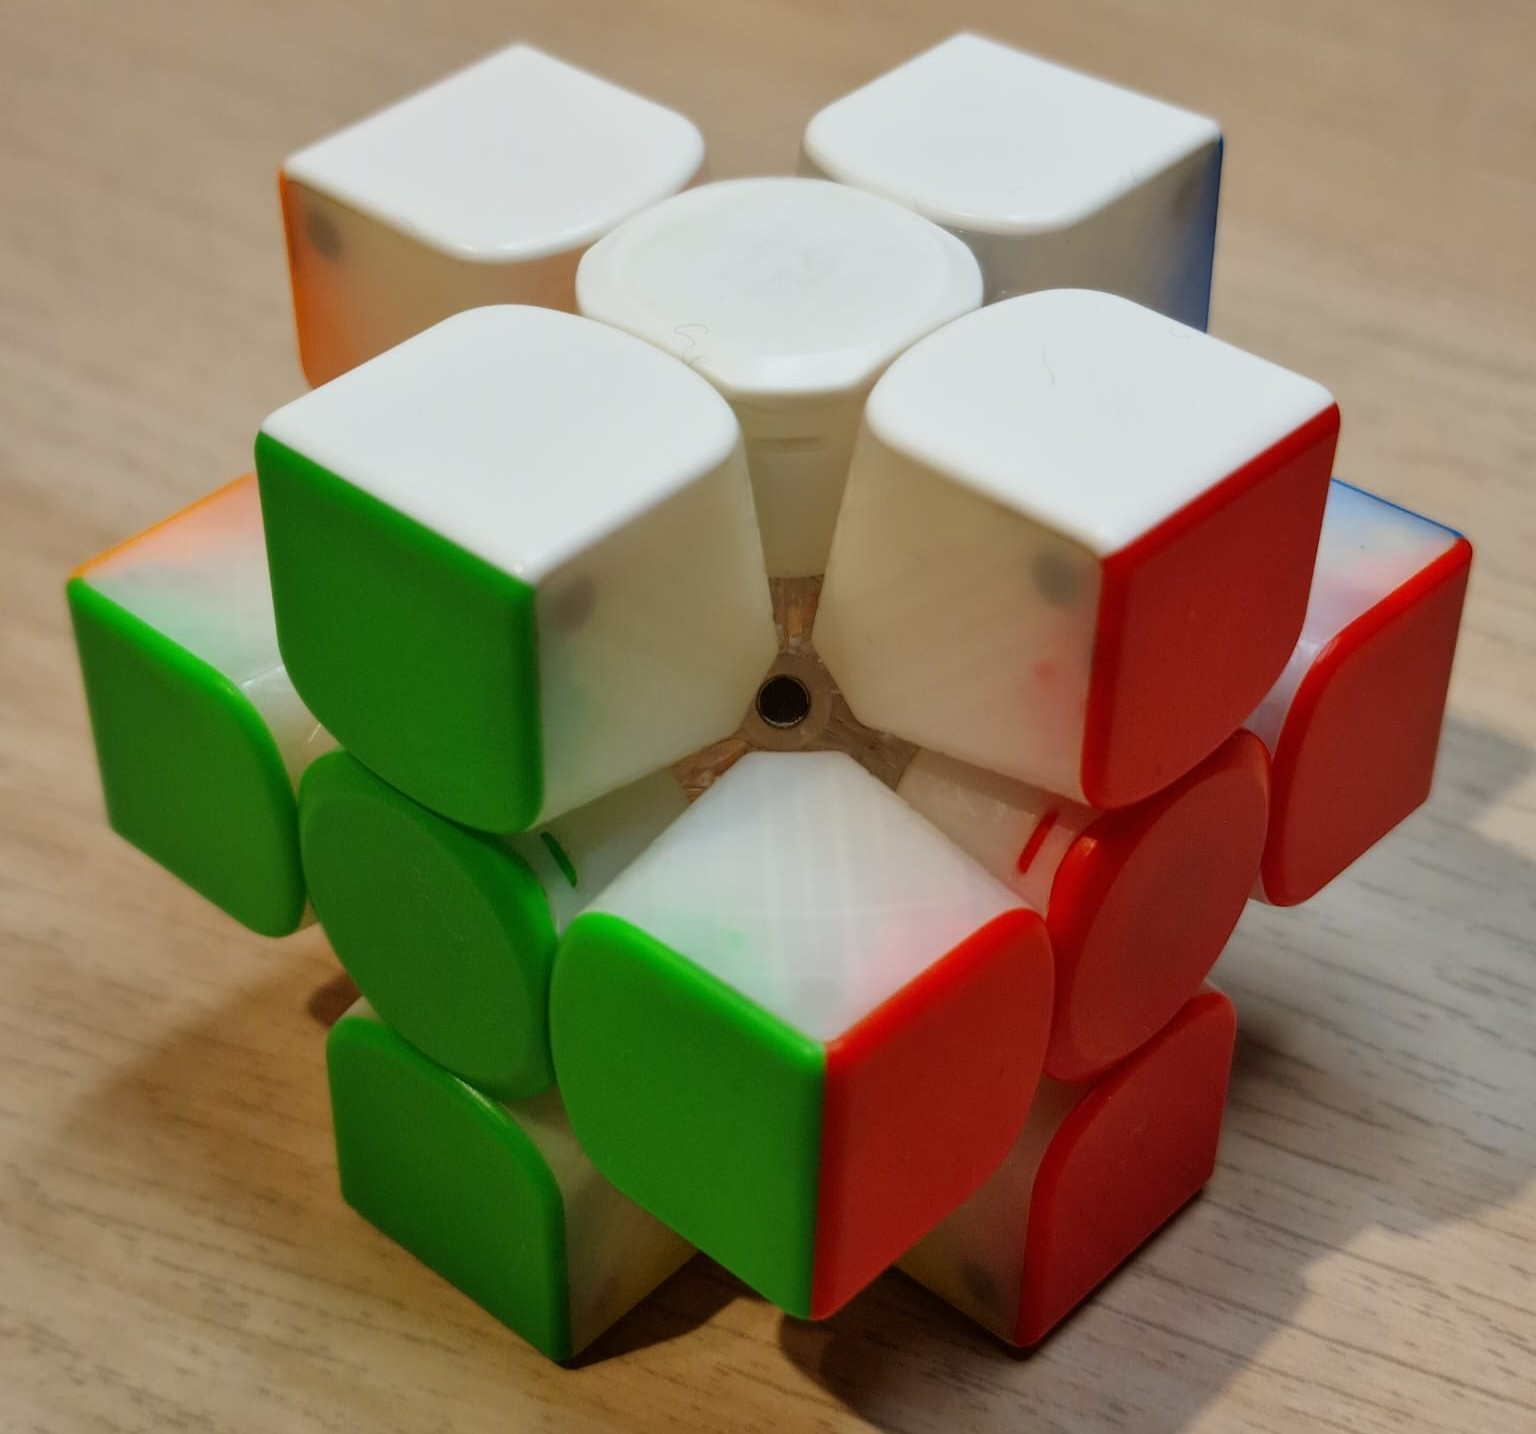
\includegraphics[width=5cm]{img/figures/only-edges.jpg}
    \caption{Cub amb només arestes}
    \label{fig:only-edges}
\end{figure} 

Llavors amb aquests càlculs podem extreure les conclusions que les combinacions possibles teòriques d'un cub de rubik són:

$$ \textrm{Nº Combinacions tèoriques} = 8!*3^8*12!*2^{12}= 519.024.039.293.878.272.000 $$
\newpage Però cal dir que aquestes no són les combinacions totals reals del cub de rubik ja que aquestes combinacions estan calculades com si demuntessim el cub com a la \ref{fig:cub-desmuntat} i recol·loquéssim les peces en un estat aleatori.
Llavors per calcular les reals s'han de dividir per 12 els casos per restriccions com les que es mostren en la següent figura.

\begin{figure}[ht]
    \centering
    \begin{minipage}[b]{0.2\textwidth}
      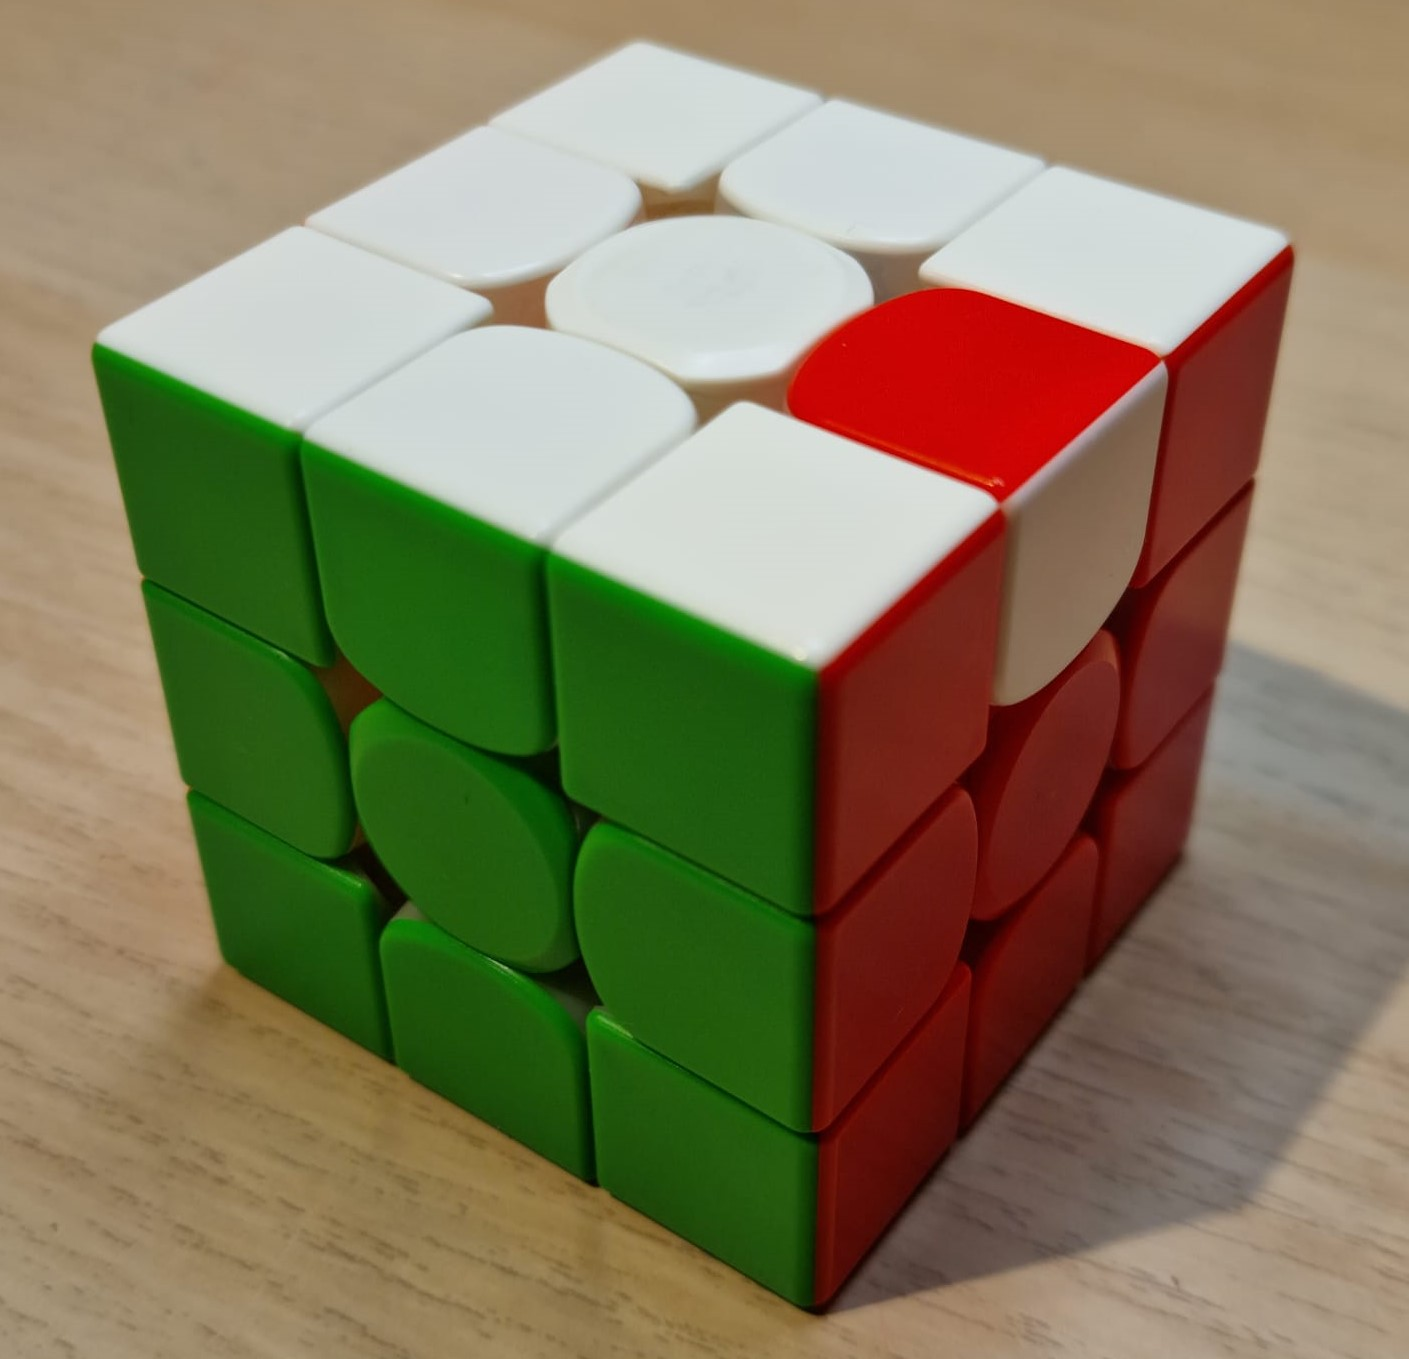
\includegraphics[width=\textwidth]{img/figures/impossible-edge.jpg}
    \end{minipage}
    \hfill
    \begin{minipage}[b]{0.2\textwidth}
      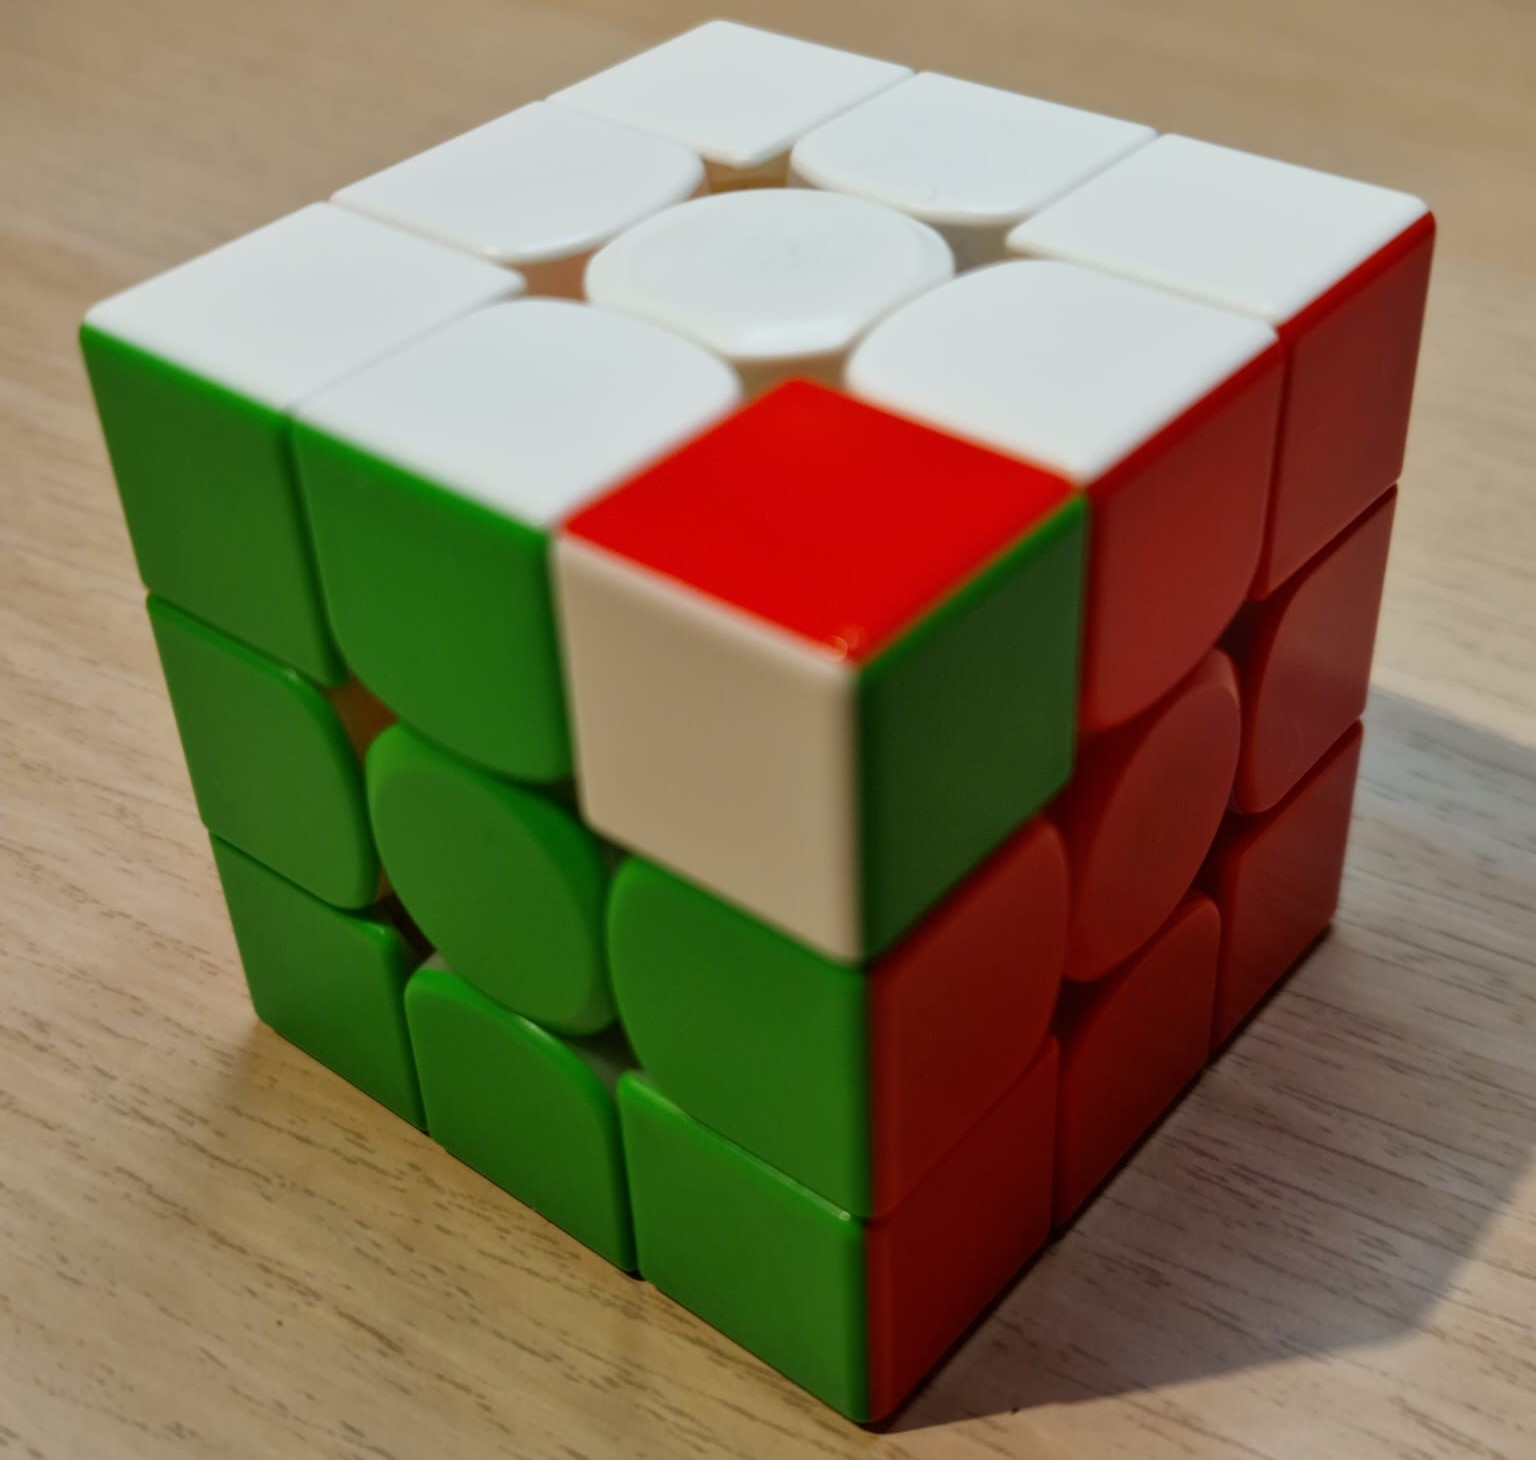
\includegraphics[width=\textwidth]{img/figures/impossible-corner.jpg}
    \end{minipage}
    \hfill
    \begin{minipage}[b]{0.2\textwidth}
        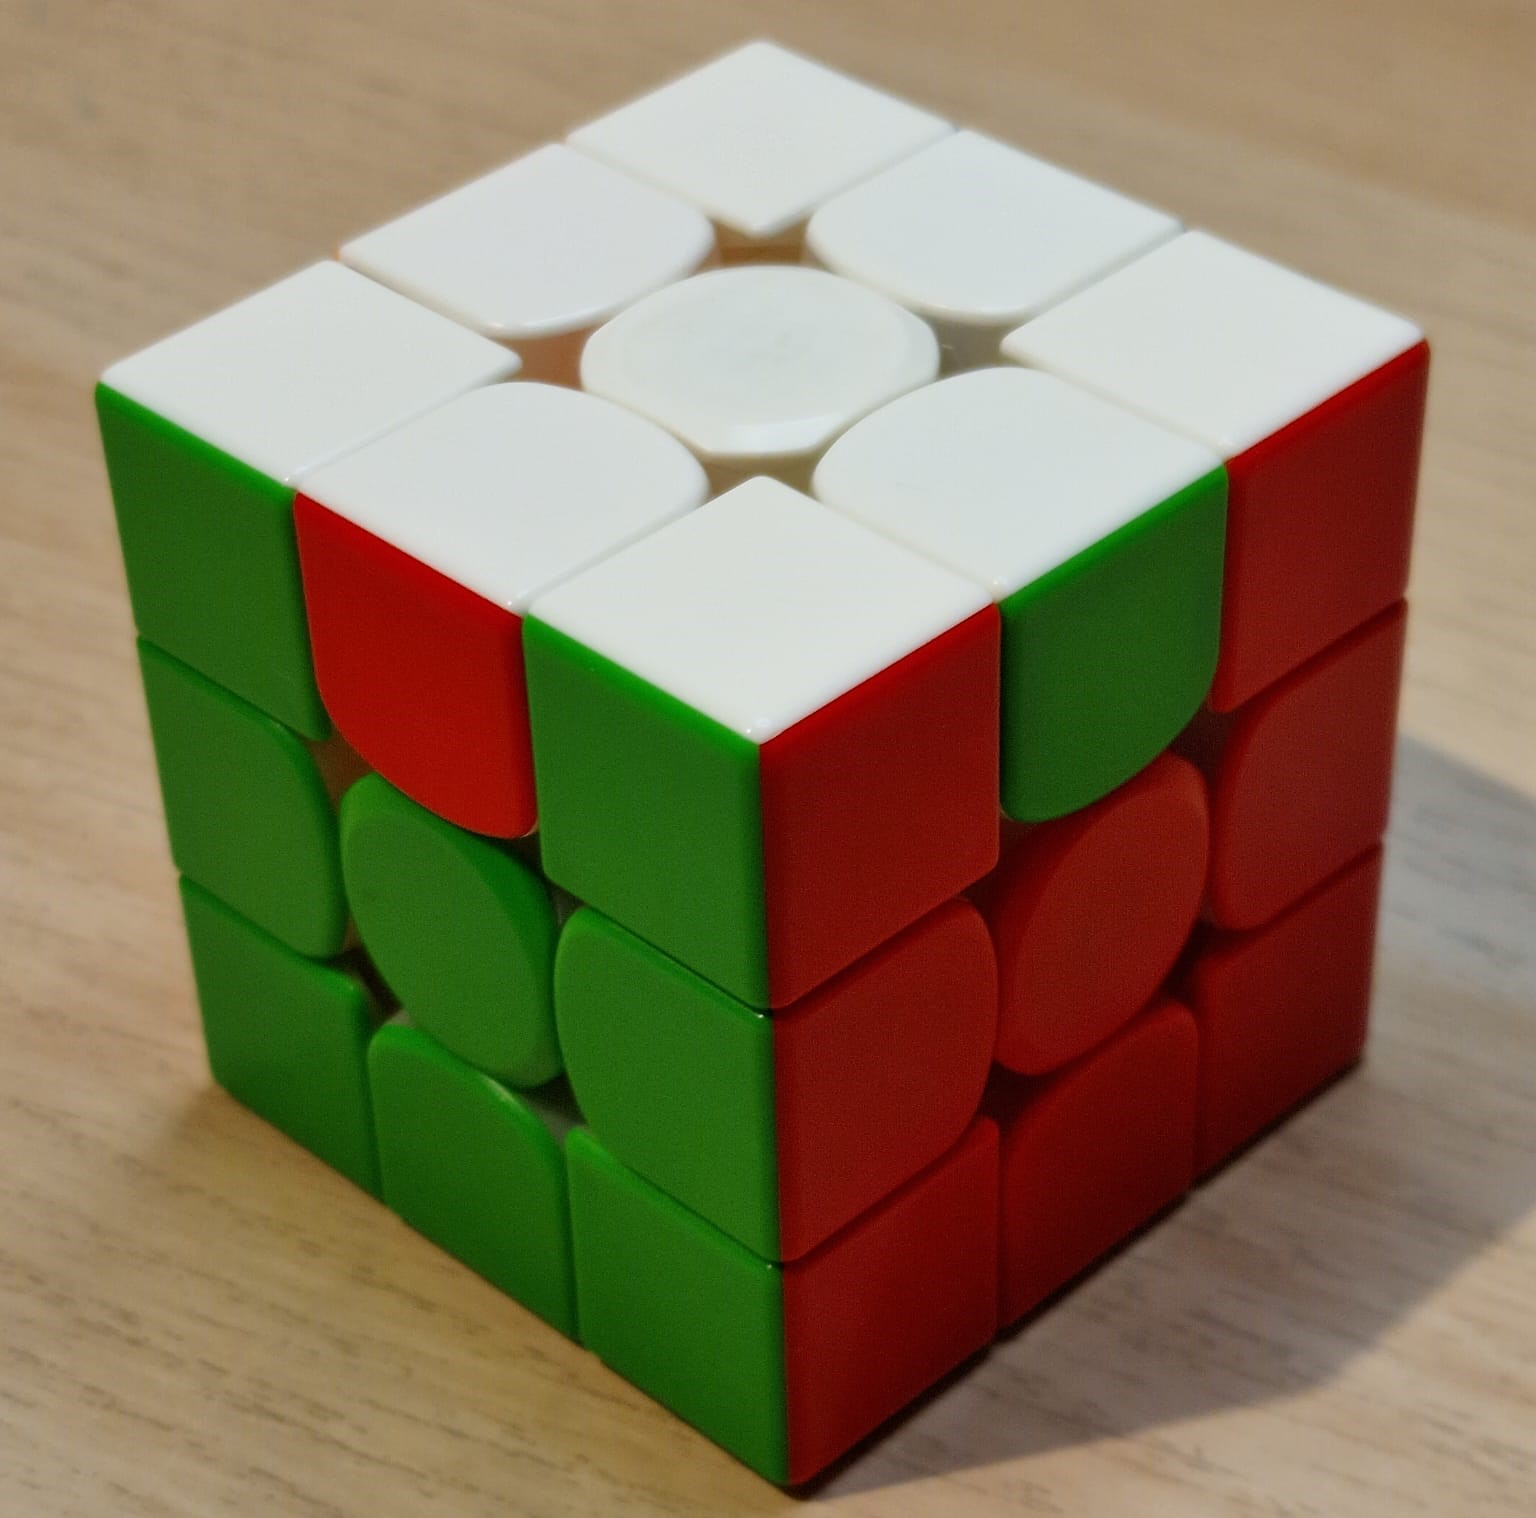
\includegraphics[width=\textwidth]{img/figures/impossible-2edge.jpg}
    \end{minipage}
    \caption{Exemple de casos impossibles}
  \end{figure}
I tot ben calculat queda:

$$ \textrm{Nº Combinacions Reals} = \frac{8!*3^8*12!*2^{12}}{12}= 43.252.003.274.489.856.000 $$

